\begin{abstract}
En el siguiente laboratorio se desarrolla un reconocedor de actividad humana el cual utiliza una un kit  Arduino Nano 33 BLE. Para esto se realiza un programa para el microcontrolador que capture la informacion del giroscopio y se envie a la computadora por el puerto USB; esta información se procesa mediante un script de python que  la guarde con etiqueta
el tipo de movimiento que se efectua y la ordene en un archivo CSV. Se registran 3 movimientos: «Up-Down», «Circle» y «Stationary». Con esta información muestrada se pretende realizar un modelo de red neuronal para cargarlo en el arduino, de modo que este pueda identificar el movimiento realizado según la red cargada con datos históricos y frecuentes para determinado movimiento. Sobre el modelo: se aspira a una red de dos capas con varias neuronas y 3 salidas (una para cada movimiento). Se entrena el modelo con el 60\% de los datos, se valida con el 20\% y se prueba con el último 20\% de los datos. Este modelo se procesa/exporta al microcontrolador mediante la librería de TensorFlow. Los practicantes se apoyan en la plataforma de EdgeImpulse para pefeccionar el modelo. El objetivo se cumplió dentro de los parámetos evaluativos. Se exporta un modelo que detectan los 3 movimientos; sobre la red neurnal no se cumplió perfectamente el objetivo el movimiento "Stationary" se predice parcialmente; pero este conocimiento no corresponde a criterios evacuativos del curso, por lo que se concluye una práctica exitosa.
\end{abstract}

Link del Proyecto: \faGithub   \hspace{0.5mm}\url{https://github.com/Jams1001/IE0624/tree/main/L5} 

\texttt{ID del último commit de interés:\href{https://github.com/Jams1001/IE0624/commit/e96a6fcf3fcca333e339f4346ee823d04a5a9c9e}{e96a6fcf3fcca333e339f4346ee823d04a5a9c9e
}}\\

\textbf{Instrucciones de simulación:}


\begin{figure}[H]
\centering
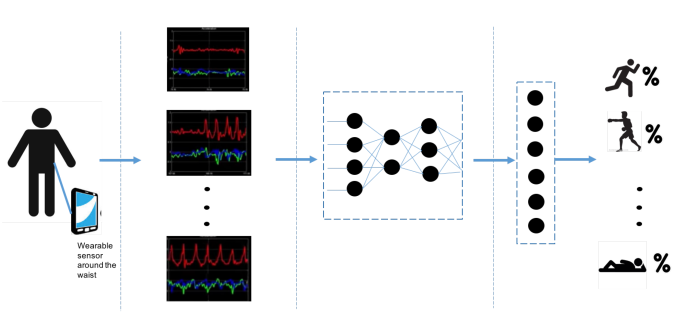
\includegraphics[scale=0.7]{./images/1.png} 
\caption{HAR.}
\label{f1}
\end{figure}
